\section{Запись речевого сигнала и исследование параметров дискретизации}
\label{sec:recording}

\subsection{Задание 1.2. Запись речи и регулировка уровней}

Запись речевого сигнала выполнялась в программе Audacity при частоте
проекта 16000 Гц, моно, разрядности 16 бит (Signed 16-bit PCM).
Тестовая фраза записана в файл \texttt{audio/lab1/1.2\_test/test.wav}.

Уровень записи регулировался с помощью регулятора громкости Windows и
ползунка усиления Audacity. Уровень считается установленным правильно,
если при произнесении фразы амплитуда на осциллограмме не превышает
значение, отмеченное красной линией индикатора (нет клиппинга), и
достаточно удалена от шума фона.

Параметры контрольной записи приведены в таблице~\ref{tab:test}.

\begin{table}[H]
	\centering
	\caption{Параметры тестовой записи \texttt{test.wav}}
	\label{tab:test}
	\begin{tabular}{|l|l|}
		\hline
		Частота дискретизации & 16000 Гц \\
		\hline
		Количество каналов & 1 (моно) \\
		\hline
		Разрядность & 16 бит (PCM) \\
		\hline
		Длительность & 15,4 с \\
		\hline
		Максимальная амплитуда (пик) & $-11{,}9$ дБFS \\
		\hline
		Клипнувшие отсчёты & 0 \\
		\hline
	\end{tabular}
\end{table}

Пик сигнала $-11{,}9$ дБFS соответствует зелёной зоне шкалы уровня:
запись достаточно громкая и не искажена. Уровень воспроизведения
проверен прослушиванием.

\subsection{Задание 1.3. Влияние частоты дискретизации и разрядности}

Для исследования влияния частоты дискретизации и разрядности на качество
и разборчивость речи из исходной записи (16 кГц, 16 бит) было
сформировано восемь производных вариантов: частоты дискретизации 4, 8, 16
и 32 кГц в сочетании с разрядностями 16 и 8 бит.

Ресемплинг выполнялся методом \texttt{resample\_poly} библиотеки SciPy
(с применением сглаживающего фильтра перед прореживанием, что исключает
частотные свёртывания). Квантование до 8 бит выполнялось по формуле
$y_q = \mathrm{round}(y \cdot 127) / 127$. Исходная запись и все
производные варианты сохранены в каталогах
\texttt{audio/lab1/1.3\_rate\_depth/original} и
\texttt{.../derived}.

Результаты расчётов приведены в таблице~\ref{tab:rate}, спектрограммы
вариантов --- на рисунке~\ref{fig:rate-spec}, осциллограммы --- на
рисунке~\ref{fig:rate-wave}.

\begin{table}[H]
	\centering
	\caption{Параметры вариантов речевого сигнала}
	\label{tab:rate}
	\begin{tabular}{|l|l|l|l|l|l|}
		\hline
		Файл & $F$, кГц & Бит & Объём, КБ & Полоса, Гц & SNR квант., дБ \\
		\hline
		phrase\_original.wav & 16 & 16 & 481,4 & 4000 & --- \\
		\hline
		phrase\_4k\_16bit.wav & 4 & 16 & 23,4 & 2000 & --- \\
		\hline
		phrase\_8k\_16bit.wav & 8 & 16 & 46,7 & 4000 & --- \\
		\hline
		phrase\_16k\_16bit.wav & 16 & 16 & 93,3 & 4000 & --- \\
		\hline
		phrase\_32k\_16bit.wav & 32 & 16 & 186,5 & 4000 & --- \\
		\hline
		phrase\_4k\_8bit.wav & 4 & 8 & 11,7 & 2000 & 27,9 \\
		\hline
		phrase\_8k\_8bit.wav & 8 & 8 & 23,4 & 4000 & 27,3 \\
		\hline
		phrase\_16k\_8bit.wav & 16 & 8 & 46,7 & 4000 & 27,0 \\
		\hline
		phrase\_32k\_8bit.wav & 32 & 8 & 93,3 & 4000 & 26,8 \\
		\hline
	\end{tabular}
\end{table}

\begin{figure}[H]
	\centering
	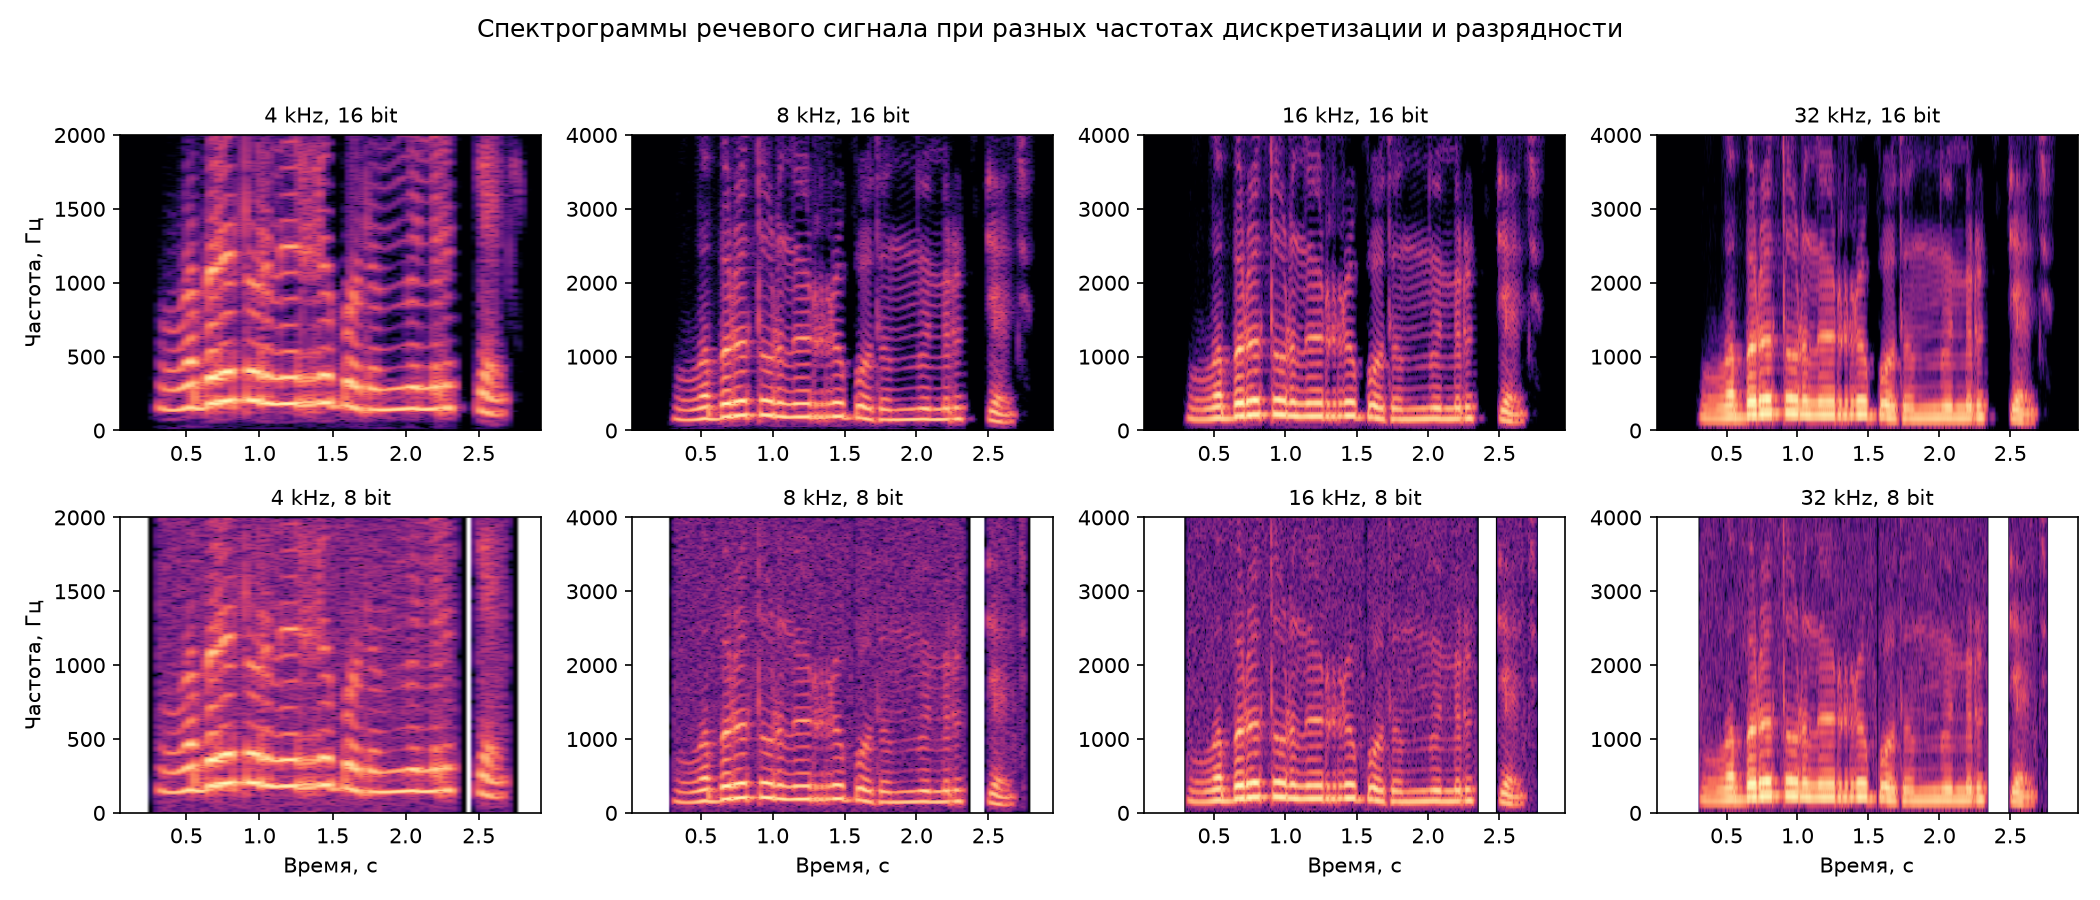
\includegraphics[width=\textwidth]{lab1_rate_bit_spectrograms.png}
	\caption{Спектрограммы речевого сигнала при разных частотах
		дискретизации и разрядности}
	\label{fig:rate-spec}
\end{figure}

\begin{figure}[H]
	\centering
	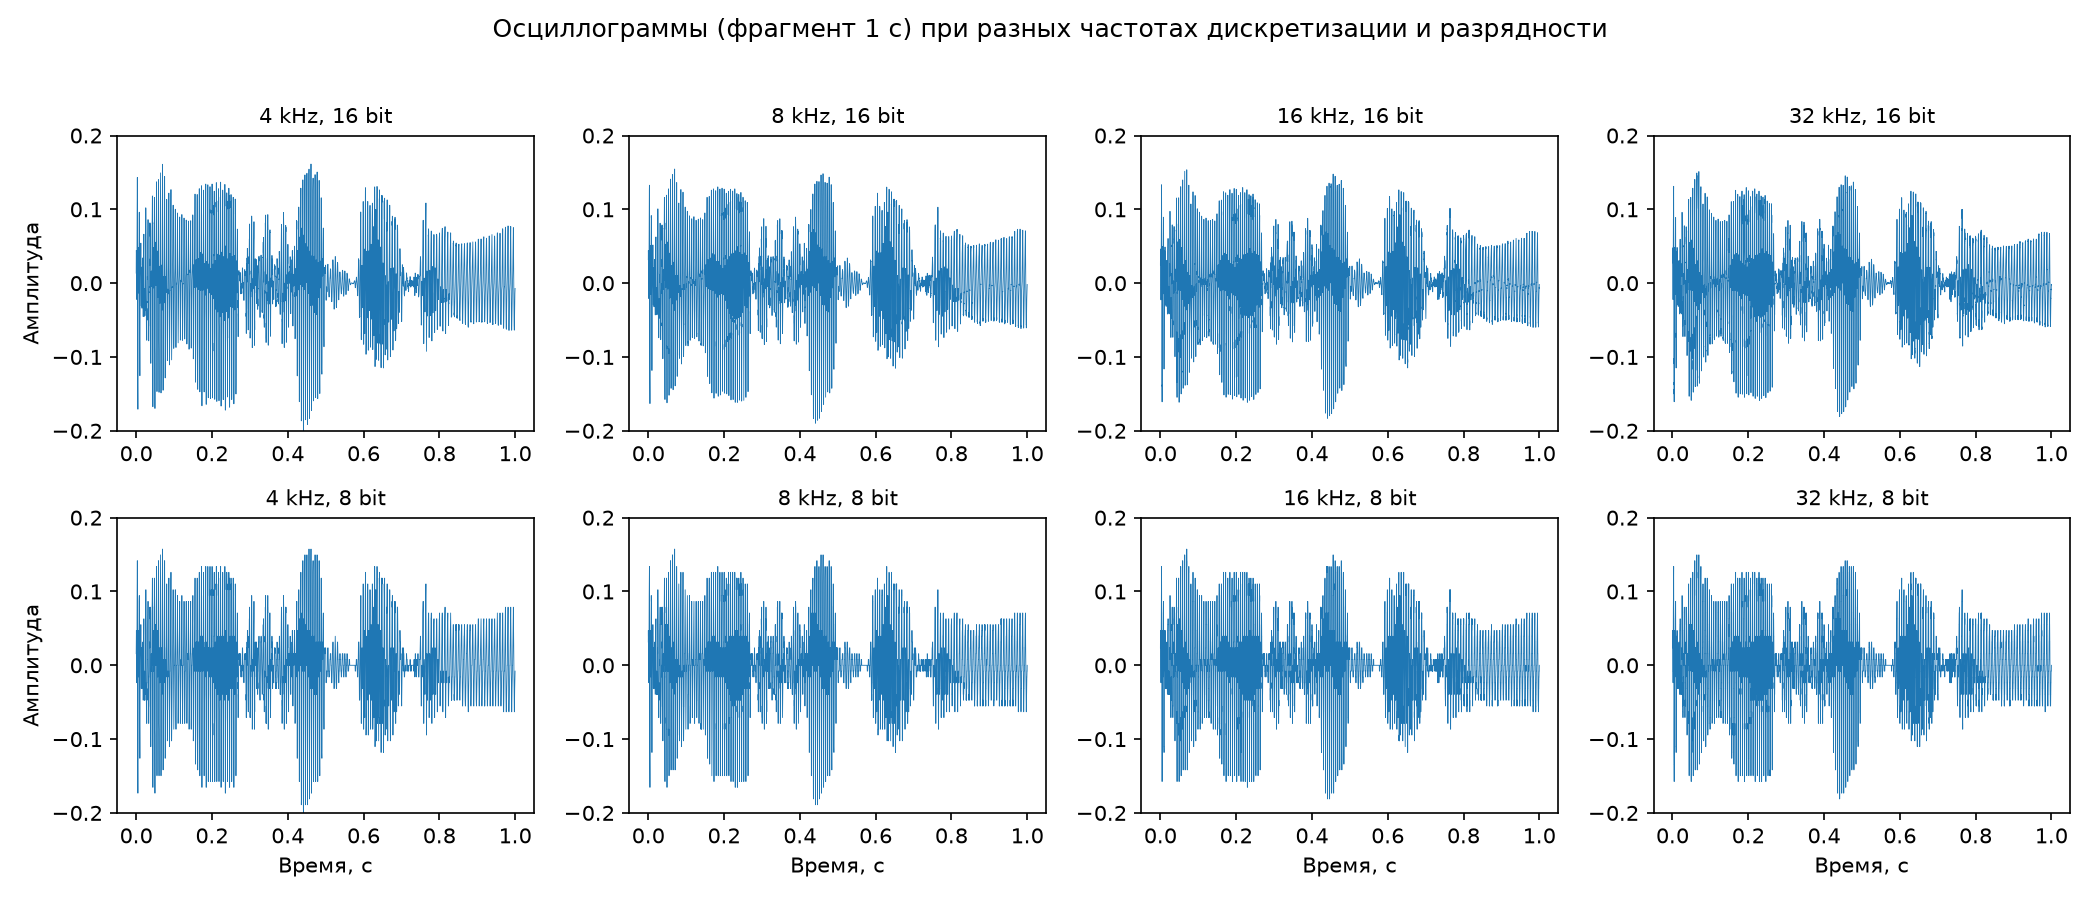
\includegraphics[width=\textwidth]{lab1_rate_bit_waves.png}
	\caption{Осциллограммы (фрагмент длительностью 1 с) при разных
		частотах дискретизации и разрядности}
	\label{fig:rate-wave}
\end{figure}

Из спектрограмм (рис.~\ref{fig:rate-spec}) наглядно видно:
\begin{itemize}
	\item при частоте дискретизации 4 кГц спектр обрезан по частоте 2 кГц
		--- часть высокочастотных компонент речи утрачена;
	\item при 8 кГц полоса составляет 4 кГц («телефонное» качество);
	\item при 16 и 32 кГц полоса речи (0--4 кГц) полностью сохранена;
	\item в 8-бит вариантах (нижняя строка) на спектрограммах виден
		ровный фон шума квантования, отсутствующий в 16-бит вариантах.
\end{itemize}

Субъективное прослушивание вариантов показало:
\begin{itemize}
	\item 16 кГц / 16 бит --- эталон качества записи;
	\item 32 кГц / 16 бит --- на слух неотличим от эталона, но объём
		файла в два раза больше;
	\item 8 кГц / 16 бит --- речь разборчива, но слышно «телефонное»
		качество;
	\item 4 кГц / 16 бит --- речь заметно приглушена, качество и
		разборчивость ухудшаются;
	\item 8-бит варианты --- на паузах и в тишине слышно шипение шума
		квантования; при этом 32 кГц / 8 бит слышится чуть лучше, чем
		16 кГц / 8 бит (при большей частоте дискретизации шум
		квантования «размазывается» по большему числу отсчётов).
\end{itemize}

Квантование до 8 бит обеспечивает SNR около 27 дБ при уровне сигнала
исходной записи; теоретический предел для равномерного квантования
составляет около 50 дБ, однако практическое значение снижено из-за того,
что речевой сигнал занимает малую часть шкалы (пик $-12$ дБFS).

\textbf{Выводы по заданию 1.3.}
\begin{enumerate}
	\item Частота дискретизации определяет полосу частот речевого
		сигнала: уменьшение частоты с 16 до 4 кГц срезает спектр до
		2 кГц и ухудшает разборчивость; 8 кГц достаточно для
		разборчивой речи (телефонное качество); 16 кГц обеспечивает
		хорошее качество; 32 кГц субъективно не даёт выигрыша для речи,
		но увеличивает объём файла в два раза.
	\item Уменьшение разрядности с 16 до 8 бит вносит шум квантования,
		слышимый на паузах, однако разборчивость речи при этом
		сохраняется.
	\item Наименьший объём при приемлемом качестве --- сочетание
		8 кГц / 8 бит; наилучшее качество --- 16 кГц / 16 бит.
\end{enumerate}
